%---------
% place your email id between the braces so that your homework has a name
\def\yourname{}
% -----------------------------------------------------
\def\duedate{4/12/24}
\def\duelocation{via \href{https://www.gradescope.com/courses/753885}{Gradescope}}
\def\hnumber{4}
\def\prof{Lorenzo Orecchia}
\def\course{\href{https://canvas.uchicago.edu/courses/56880}{CMSC 27200 - Spring 2024}}
%-------------------------------------

\documentclass[10pt]{article}
\usepackage[colorlinks,urlcolor=blue]{hyperref}
\usepackage[osf]{mathpazo}
\usepackage{amsmath,amsfonts,graphicx}
\usepackage{latexsym}
%\usepackage{subfig}
\usepackage{algpseudocode}
\usepackage[shortlabels]{enumitem}
\usepackage{algorithm}
\usepackage{listings}

\usepackage{tikz}
\usepackage{qtree}
\usepackage{tikz-qtree}
\usepackage{subcaption}
\usepackage{float}   

%\usepackage[top=1in,bottom=1.4in,left=1.5in,right=1.5in,centering]{geometry}
\usepackage{fullpage}
\usepackage{color}
\definecolor{mdb}{rgb}{0.3,0.02,0.02} 
\definecolor{cit}{rgb}{0.05,0.2,0.45}
\usepackage{wrapfig}
%\pagestyle{myheadings}
\markboth{\yourname}{\yourname}

\thispagestyle{empty}

\newenvironment{proof}{\par\noindent{\it Proof.}\hspace*{1em}}{$\Box$\bigskip}
\newcommand{\qed}{$\Box$}
\newcommand{\alg}[1]{\mathsf{#1}}
\newcommand{\handout}{
   \renewcommand{\thepage}{H\hnumber-\arabic{page}}
   \noindent
   \begin{center}
      \vbox{
    \hbox to \columnwidth {\sc{\course} --- \prof \hfill}
    \vspace{-2mm}
    \hbox to \columnwidth {\sc due \MakeLowercase{\duedate} \duelocation\hfill {\Huge\color{mdb}H\hnumber.\yourname}}
      }
   \end{center}
   \vspace*{2mm}
}
\newcommand{\solution}[1]{
\vspace{2mm}

\noindent Collaborators:

\vspace{5mm}

\medskip\noindent{\color{cit}\textbf{Solution:} #1}}

\newcommand{\bit}[1]{\{0,1\}^{ #1 }}
\newcommand{\extraspace}{\medskip\noindent{\color{cit} Extra space for your solution}\newpage}
%\dontprintsemicolon
%\linesnumbered=
\newtheorem{problem}{\sc\color{cit}Problem}
\newtheorem{lemma}{Lemma}
\newtheorem{theorem}{Theorem}
\newtheorem{definition}{Definition}
\newtheorem{claim}{Claim}


\begin{document}
\handout
\begin{itemize}
\item The assignment is due at Gradescope on \duedate.

\item A LaTeX template will be provided for each homework. You are strongly encouraged to type your homework into this template using \LaTeX.  If you are writing by hand, please fill in the solutions in this template, inserting additional sheets as necessary. This will help facilitate the grading.

\item You are permitted to discuss the problems with up to 2 other students in the class (per problem); however, {\em you must write up your own solutions, in your own words}. Do not submit anything you cannot explain. If you do collaborate with any of the other students on any problem, please list all your collaborators in the appropriate spaces.

\item Similarly, please list any other source you have used for each problem, including other textbooks or websites.

\item {\em Show your work.} Answers without justification will be given little credit.

\item Your homework is \textit{resubmittable}. Please refer to the course syllabus on Canvas for a more detailed description of this. For any problem that you have not changed from your last submission, please make sure to indicate this in your submission to help our graders grade faster. 

\item Is anyone still reading these?

\end{itemize}

%%%%%%%%%%%%%%%%%%%%%%%%%%%%%%%%%%%%%%%%%%%

%%%%%%%%%%%%%%%%%%%%%%%%%%%%%%%%%%%%%%%%%%%

\newpage
\begin{problem}[Linear Algebra Practice]
This question is on the basics of linear algebra, please write out all steps for computation and formal proofs:
\begin{enumerate}[(a)]
    \item Let $A = \begin{pmatrix} 2 & 5 \\ 1 & 3 \end{pmatrix}$, compute the following:
    \begin{enumerate}[(i)]
        \item $A^{-1}$
        \item $A^T$
        \item $A^2$
    \end{enumerate}
    \item Let $A$ and $B$ be $n\times n$ matrices. What's wrong with the equation $(A+B)^2 = A^2 + 2AB + B^2$? Prove that the above equation holds if and only if $A$ and $B$ commute.
    \item Let $A$ be a $n \times m$ matrix. Consider function $f: \mathbb{R}^n \rightarrow \mathbb{R}^m$ where $f(x) = Ax$. Formally prove that $f$ is a linear map (i.e. you need to show that $f(ax+by) = af(x) + bf(y)$ for all $x, y \in \mathbb{R}^n$ and $a, b \in \mathbb{R}$).
\end{enumerate}
    
\end{problem}

\begin{solution}

    \begin{enumerate}[(a)]

        \item {
            \begin{enumerate}[(i)]
                \item {
                    
                    $\displaystyle
                    A^{-1}
                    = \frac{1}{2 \cdot 3 - 5 \cdot 1} \begin{pmatrix} 3 & -5 \\ -1 & 2 \end{pmatrix}
                    = \begin{pmatrix} 3 & -5 \\ -1 & 2 \end{pmatrix}
                    $

                }
                \item {
                    $\displaystyle
                    A^{T}
                    = \begin{pmatrix} 2 & 1 \\ 5 & 3 \end{pmatrix}
                    $
                }
                \item {
                    $\displaystyle
                    A^2 
                    = \begin{pmatrix} 2 & 5 \\ 1 & 3 \end{pmatrix} \cdot \begin{pmatrix} 2 & 5 \\ 1 & 3 \end{pmatrix}
                    = \begin{pmatrix} 2 \cdot 2 + 5 \cdot 1 & 2 \cdot 5 + 5 \cdot 3 \\ 1 \cdot 2 + 3 \cdot 1 & 1 \cdot 5 + 3 \cdot 3 \end{pmatrix}
                    = \begin{pmatrix} 9 & 25 \\ 5 & 14 \end{pmatrix}
                    $
                }
            \end{enumerate}
        }
        \item {
            The equation assumes $A$ and $B$ commute. 
            
            $\implies \\
            (A+B)^2 = A^2 + 2AB + B^2 \\
            A^2 + AB + BA + B^2 = A^2 + 2AB + B^2 \\
            BA = AB
            $

            $\impliedby \\
            BA = AB \\
            BA + AB = 2AB \\
            A^2 + BA + AB + B^2 = A^2 + 2AB + B^2 \\
            (A+B)^2 = A^2 + 2AB + B^2 \\
            $
        }
        \item {
            $f(ax+by) = A \cdot (ax + by) = A \cdot (ax) + A \cdot (by) = a \cdot Ax + b \cdot Ay = af(x) + bf(y)$
        }

    \end{enumerate}
    
\end{solution}

\newpage

%%%%%%%%%%%%%%%%%%%%%%%%%%%%%%%%%%%%%%%%%%%

%%%%%%%%%%%%%%%%%%%%%%%%%%%%%%%%%%%%%%%%%%%

\begin{problem}[Modular FFT]
This question is based on problem 2.30 from [DPV].

This problem illustrates how to do the Fourier Transform (FT) in modular arithmetic, for example, modulo 7.
\begin{enumerate}
    \item[(a)] There is at least one number $\omega$ such that all the powers $\omega$, $\omega^2$,..., $\omega^6$ are distinct (modulo $7$). Find one such $\omega$, and show that $\omega$ + $\omega^2$ + · · · + $\omega^6 \equiv 0 \mod 7$. (Interestingly, for any prime modulus there is such a number.)
    \item[(b)] Using the matrix form of the FT, produce the transform of the sequence $(0,1,1,1,5,2)$ modulo $7$; that is, multiply this vector by the $6\times 6$ matrix $M_6(\omega)$, for the value of $\omega$ you found earlier. In the matrix multiplication, all calculations should be performed modulo 7.
    \item[(c)] Write down the matrix necessary to perform the inverse FT. Recall that dividing by a number amounts to multiplying by its inverse. Show that multiplying by this matrix returns the original sequence. (Again all arithmetic should be performed modulo 7.)
    \item[(d)] Now show how to multiply the polynomials $x^2 + x + 1$ and $x^3 + 2x - 1$ using the FT modulo 7.
\end{enumerate}
\end{problem}
\begin{solution}

    \begin{enumerate}[(a)]
        \item {
            $\omega = 3$

            $\omega \equiv_7 3$ \\
            $\omega^2 \equiv_7 2$ \\
            $\omega^3 \equiv_7 6$ \\
            $\omega^4 \equiv_7 4$ \\
            $\omega^5 \equiv_7 5$ \\
            $\omega^6 \equiv_7 1$ 

            $\omega + \omega^2 + \dots + \omega^6 \equiv_7 3 + 2 + 6 + 4 + 5 + 1 \equiv_7 0$
        }
        \item {
            \begin{flalign*}
                \displaystyle
                \begin{pmatrix}
                    1 & 1 & 1 & 1 & 1 & 1 \\
                    1 & w & w^2 & w^3 & w^4 & w^5 \\
                    1 & w^2 & w^4 & w^6 & w^8 & w^{10} \\
                    1 & w^3 & w^6 & w^9 & w^{12} & w^{15} \\
                    1 & w^4 & w^8 & w^{12} & w^{16} & w^{20} \\
                    1 & w^5 & w^{10} & w^{15} & w^{20} & w^{25} \\
                \end{pmatrix} \cdot
                \begin{pmatrix} 
                    0 \\ 1 \\ 1 \\ 1 \\ 5 \\ 2 
                \end{pmatrix}
                &\equiv_7
                \begin{pmatrix}
                    1 & 1 & 1 & 1 & 1 & 1 \\
                    1 & 3 & 2 & 6 & 4 & 5 \\
                    1 & 2 & 4 & 1 & 2 & 4 \\
                    1 & 6 & 1 & 6 & 1 & 6 \\
                    1 & 4 & 2 & 1 & 4 & 2 \\
                    1 & 5 & 4 & 6 & 2 & 3
                \end{pmatrix} \cdot
                \begin{pmatrix} 
                    0 \\ 1 \\ 1 \\ 1 \\ 5 \\ 2 
                \end{pmatrix}
                \\
                &\equiv_7
                \begin{pmatrix} 
                    0 + 1 + 1 + 1 + 5 + 2 \\
                    0 + 3 + 2 + 6 + 20 + 10 \\
                    0 + 2 + 4 + 1 + 10 + 8 \\
                    0 + 6 + 1 + 6 + 5 + 12 \\
                    0 + 4 + 2 + 1 + 20 + 4 \\
                    0 + 5 + 4 + 6 + 10 + 6
                \end{pmatrix}
                \\
                &\equiv_7
                \begin{pmatrix} 
                    3 \\
                    6 \\
                    4 \\
                    2 \\
                    3 \\
                    3
                \end{pmatrix}
            \end{flalign*}
        }
        \item {
            Use formula for Vandermond inverse using modular inverse of $\omega$, $5$:

            \begin{flalign*}
                M_6^{-1}(\omega)
                &\equiv_7
                6^{-1} M_6(\omega^{-1})
                \\
                &\equiv_7
                6
                \begin{pmatrix}
                    1 & 1 & 1 & 1 & 1 & 1 \\
                    1 & 5 & 5^2 & 5^3 & 5^4 & 5^5 \\
                    1 & 5^2 & 5^4 & 5^6 & 5^8 & 5^{10} \\
                    1 & 5^3 & 5^6 & 5^9 & 5^{12} & 5^{15} \\
                    1 & 5^4 & 5^8 & 5^{12} & 5^{16} & 5^{20} \\
                    1 & 5^5 & 5^{10} & 5^{15} & 5^{20} & 5^{25} \\
                \end{pmatrix}
                \\
                &\equiv_7
                \begin{pmatrix}
                    6 & 6 & 6 & 6 & 6 & 6 \\
                    6 & 4 & 5 & 1 & 3 & 2 \\
                    6 & 5 & 3 & 6 & 5 & 3 \\
                    6 & 1 & 6 & 1 & 6 & 1 \\
                    6 & 3 & 5 & 6 & 3 & 5 \\
                    6 & 2 & 3 & 1 & 5 & 4 \\
                \end{pmatrix}
            \end{flalign*}

            Check inversion:

            \begin{flalign*}
                \begin{pmatrix}
                    6 & 6 & 6 & 6 & 6 & 6 \\
                    6 & 2 & 3 & 1 & 5 & 4 \\
                    6 & 3 & 5 & 6 & 3 & 5 \\
                    6 & 1 & 6 & 1 & 6 & 1 \\
                    6 & 5 & 3 & 6 & 5 & 3 \\
                    6 & 4 & 5 & 1 & 3 & 2 \\
                \end{pmatrix} \cdot 
                \begin{pmatrix} 
                    3 \\
                    6 \\
                    4 \\
                    2 \\
                    3 \\
                    3
                \end{pmatrix}
                &\equiv_7
                \begin{pmatrix} 
                    0 \\
                    1 \\
                    1 \\
                    1 \\
                    5 \\
                    2
                \end{pmatrix}
            \end{flalign*}
        }
        \item {
            $M_6(\omega)$ is a linear transformation from the coefficient basis to the value basis. 
            $M_6^{-1}(\omega)$ the inverse, a linear transformation from the value basis to the coefficient basis. 

            In the value basis, polynomial multiplication is equivalent to element-wise multiplication. 
            
            Let $p_1 = x^2+x+1$ and $p_2 = x^3+2x-1$. 
            Under the coefficient basis representation, we have:

            \[
                \vec{p_1} = 
                \begin{pmatrix} 
                    1 \\
                    1 \\
                    1 \\
                    0 \\
                    0 \\
                    0
                \end{pmatrix}
                \quad\quad\quad
                \vec{p_2} = 
                \begin{pmatrix} 
                    -1 \\
                    2 \\
                    0 \\
                    3 \\
                    0 \\
                    0
                \end{pmatrix}
            \]

            Tranforming to the value basis gives:

            \[
                M_6(\omega) \cdot \vec{p_1} \equiv_7
                \begin{pmatrix} 
                    3 \\
                    6 \\
                    0 \\
                    1 \\
                    0 \\
                    3
                \end{pmatrix}
                \quad\quad\quad
                M_6(\omega) \cdot \vec{p_2} \equiv_7
                \begin{pmatrix} 
                    2 \\
                    4 \\
                    4 \\
                    3 \\
                    1 \\
                    1
                \end{pmatrix}
            \]

            Then the value basis representation for the polynomial product $p_1 \cdot p_2 = p_{1 \cdot 2}$ given by:

            \[
                M_6(\omega) \cdot \vec{p_{1 \cdot 2}} = 
                (M_6(\omega) \cdot \vec{p_1}) \odot (M_6(\omega) \cdot \vec{p_2}) \equiv_7
                \begin{pmatrix} 
                    6 \\
                    3 \\
                    0 \\
                    3 \\
                    0 \\
                    3
                \end{pmatrix}
            \]

            Tranform back to coefficient basis to get $p_{1 \cdot 2}$'s coefficients:

            \[
                \vec{p_{1 \cdot 2}} =
                M_6^{-1}(\omega) \cdot
                \begin{pmatrix} 
                    6 \\
                    3 \\
                    0 \\
                    3 \\
                    0 \\
                    3
                \end{pmatrix} \equiv_7
                \begin{pmatrix} 
                    6 \\
                    1 \\
                    1 \\
                    3 \\
                    1 \\
                    1
                \end{pmatrix}
            \]

            So $p_1 \cdot p_2 \equiv_7 x^5 + x^4 + 3x^3 + x^2 + x + 6$. 
        }
    \end{enumerate}

\end{solution}

\newpage


%%%%%%%%%%%%%%%%%%%%%%%%%%%%%%%%%%%%%%%%%%%

%%%%%%%%%%%%%%%%%%%%%%%%%%%%%%%%%%%%%%%%%%%

\begin{problem}[Bipartite Graphs]
This question is similar to question 3.7 in [DPV].

A bipartite graph is an undirected graph $G=(V,E)$ whose vertex set $V$ can be partitioned into two sets $V_1$ and $V_2$ (i.e. $V = V_1 \cup V_2$ and $V_1 \cap V_2 = \emptyset$) such that there are no edges between vertices of the same set. In other words, all edges are of the form $(u,v)$, where $u \in V_1$ and $v \in V_2$.

\begin{enumerate}
    \item[(a)]Sketch a proof that a graph is bipartite if and only if it contains no odd cycle.
    \item[(b)]Give an $O(|V|+|E|)$ time algorithm with pseudocode to check if a graph is bipartite, and formally prove that it is correct and that it runs in $O(|V|+|E|)$ time. 
\end{enumerate}
\end{problem}
\begin{solution}
    
    \begin{enumerate}[(a)]
        \item {
            \begin{proof}

                Let $G = (V, E)$ be a bipartite graph with bipartitions $V_1$ and $V_2$. 

                $\implies$

                If $G$ is bipartite, then all odd length paths starting in one bipartition must end in the other bipartition, 
                because there are no edges between vertices in the same bipartition. 

                Cycle are paths that start and end in the same bipartition, so they cannot have odd length. 

                $\impliedby$

                Suppose no odd cycle exists in G. 

                Let $r \in V$ be an arbitrary vertex. 
                Let $V_e$ and $V_o$ be the sets of vertices in $V$ whose shortest path to $r$ is of even and odd length, respectively. 
                By construction, $V_e$ and $V_o$ must be disjoint. 
                We claim $(V_e, V_o)$ is a valid bipartition of G.

                Suppose for contradiction that there exists $(u, v) \in E$ such that $u, v$ are in the same bipartition. 
                Let $P_{r \rightarrow u}$ and $P_{r \rightarrow v}$ be the shortest paths from $r$ to $u$ and $r$ to $v$, respectively. 
                $P_{r \rightarrow u}$ and $P_{r \rightarrow v}$ must either both be of odd length, or both be of even length. 
                Thus, with $(u, v)$, $W = P_{r \rightarrow u} \cup P_{r \rightarrow v}$ is a closed walk of odd length. 
                
                If $r$ is the only repeated vertex in $W$, then $W$ is an odd cycle. 

                Otherwise, there exists $v_i, v_j \in W$ such that $v_i = v_j$. 
                There then exists a closed walk $v_i \rightarrow v_j$ along with the closed walk $r \rightarrow r$. 
                One of these must be odd and the other even. 
                Repeating this gives an odd cycle. 

                Thus, we have a contradiction. 
            \end{proof}
        }
        \item{
            \begin{algorithm}[H]
                \caption{Breadth-first search algorithm looking for odd cycles}
                \begin{algorithmic}[1]
                    \Statex \textbf{$bipartite(G, v)$}
                    \Statex \textbf{Input:} $G, r \in V$
                    \Statex \textbf{Output:} $\mathcal{T/F}$
                    
                    \State $dist(\forall V) = \infty$
                    \State $dist(r) = 0$

                    \State $Q \gets Queue[r]$

                    \While{$|Q| \geq 1$}
                        \State $v \gets Q.dequeue$

                        \For{$u \in adj(v)$}
                            \State \textbf{if $dist(u) = \infty$ then} 
                            \State \quad $Q.enqueue(u)$
                            \State \quad $dist(u) = dist(v) + 1$
                            \State \textbf{else if } $(length(u) + length(v) + 1)$ is $odd$ \textbf{then}
                            \State \quad \textbf{return $\mathcal{F}$} 
                        \EndFor
                    \EndWhile

                    \State \textbf{return $\mathcal{T}$}

                \end{algorithmic}
            \end{algorithm}

            \begin{proof}

                First, we prove that the algorithm computes the lengths of 
                shortest paths from $r$ using induction on their lengths. Here, 
                we assume the graph is connected. 

                In the base case, for length $0$, $dist(r)$ is initialized to $0$. 

                In the inductive case, assume the algorithm correctly computes 
                shortest path lengths up to length $\ell$. 
                Then consider a vertex $v$ at shortest distance $\ell + 1$ from 
                $r$. 
                Because this distance is finite, there must exist a path from 
                $r$ to $v$, so $v$ must have a neighbor $u$ a shortest distance 
                $\ell$ from $r$. 
                By the inductive hypothesis $u$'s shortest distance was 
                correctly determined. 
                The algorithm gets the shortest distance of $v$ by adding one to 
                that of $u$, since they are neighbors and a queue is used. 

                Thus, the shortest distances are correctly determined. 

                Now, at each step the algorithm also checks if a closed walk was 
                created. 
                Note that this step does not affect the state of the BFS. 
                If a closed walk is detected, our correct computation of the 
                shortest distances allows a correct computation of the walk 
                length. 
                If the walk is odd, then by (a) there also exists an odd cycle 
                so the graph is not bipartite. 
                If no such cycle is detected then the graph is bipartite. 

            \end{proof}

            \begin{proof}

                This algorithm is a modification of BFS. 
                Each vertex and edge is considered a constant number of times. 
                The cycle checking step is also constant, as the distances are 
                already computed. 
                So, the algorithm is $O(|V|+|E|)$. 

            \end{proof}
        }

    \end{enumerate}

\end{solution}
\newpage

%%%%%%%%%%%%%%%%%%%%%%%%%%%%%%%%%%%%%%%%%%%

%%%%%%%%%%%%%%%%%%%%%%%%%%%%%%%%%%%%%%%%%%%

\begin{problem}[Verifying Binary Search Trees]
For this problem you may assume that a binary tree node is defined as follows:

\begin{verbatim}
class node:
    left: node = None
    right: node = None
    value
\end{verbatim}
You can assume that the values are distinct and the value type supports comparison.
A binary tree $T$ is called a binary search tree (BST) if and only if \textbf{for every node V} in the tree
\[\max_{U \in V.left} U.val < V.val < \min_{W \in V.right} W.val\]

\begin{enumerate}[(a)]
    \item Write pseudocode for a \textbf{recursive} algorithm that takes as input the root $T$ of a binary tree and returns whether it is a BST. Your algorithm can optionally return more than just a boolean value. You are allowed to define helper functions if you want. Your algorithm should run in $O(n)$ time, where $n$ is the number of nodes in tree $T$.

    \item Prove the correctness of your algorithm.
\end{enumerate}
The height of a tree is defined as 
\[height(T) = \begin{cases} 0 & T = None \\
1 + \max\big(height(T.left), height(T.right)\big) & \text{o.w.}\end{cases}\]
We would like all our Binary Search Trees operations (look-up, insertion, deletion) to have $O(\log n)$ time complexity. To achieve that, we require the BST to also be \textbf{balanced}.
A BST is balanced if and only if \textbf{for every node V} in the tree
\[\big|height(V.left) - height(V.right)\big| \leq 1\]

\begin{enumerate}[(a),resume]
    \item Modify below your pseudocode from part (a) to check if the binary tree $T$ is a \textbf{balanced} BST. Your modified algorithm should also have $O(n)$ time complexity.
\end{enumerate}
\end{problem}

\begin{figure}[ht]
    \centering
    \begin{subfigure}[b]{0.3\textwidth}
        \centering
        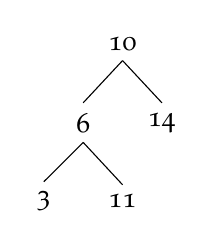
\begin{tikzpicture}[level distance=1cm,
                            level 1/.style={sibling distance=1cm},
                            level 2/.style={sibling distance=1cm}]
            \node {10}
                child {node {6}
                    child {node {3}}
                    child {node {11}}
                }
                child {node {14}};
        \end{tikzpicture}
        \caption{This is not a BST since $11 > 10$}
    \end{subfigure}
    \begin{subfigure}[b]{0.3\textwidth}
        \centering
        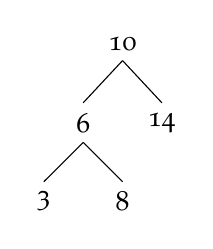
\begin{tikzpicture}[level distance=1cm,
                            level 1/.style={sibling distance=1cm},
                            level 2/.style={sibling distance=1cm}]
            \node {10}
                child {node {6}
                    child {node {3}}
                    child {node {8}}
                }
                child {node {14}};
        \end{tikzpicture}
        \caption{This is a balanced BST}
    \end{subfigure}
    \begin{subfigure}[b]{0.3\textwidth}
        \centering
        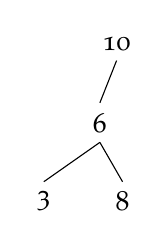
\begin{tikzpicture}[level distance=1cm,
                            level 1/.style={sibling distance=1cm},
                            level 2/.style={sibling distance=1cm}]
            \node {10}
                child[left] {node {6}
                    child {node {3}}
                    child {node {8}}
                };
        \end{tikzpicture}
        \caption{This is a BST, but not balanced}
    \end{subfigure}
\end{figure}

\begin{solution}

    \begin{enumerate}[(a)]
        \item {
            Define 2 helper functions. 
            
            \begin{algorithm}[H]
                \caption{Binary Tree Validation Algorithm}
                \begin{algorithmic}[1]
                    \Statex isBST(low, v, high)
                    \Statex \textbf{Input:} $v \in V$; $low, high \in \mathbb{R}$
                    \Statex \textbf{Output:} T/F
                    
                    \State \textbf{if $v = None$ return $T$}
                    \State \textbf{if $low \neq None$ and $v.val < low$ then return $F$}
                    \State \textbf{if $high \neq None$ and $v.val > high$ then return $F$}
                    \State \textbf{if not $isBST(low, v.left, v.val)$ then return $F$}
                    \State \textbf{if not $isBST(v.val, v.right, high)$ then return $F$}
                    \State \textbf{return $T$}

                \end{algorithmic}
                \begin{algorithmic}[1]
                    \Statex isBST(v)
                    \Statex \textbf{Input:} Root $v$
                    \Statex \textbf{Output:} T/F
                    
                    \State \textbf{return $isBST(None, v, None)$}
    
                \end{algorithmic}
            \end{algorithm}
        }
        \item {
            \begin{proof}

                We use induction on $n$, the size of the tree. 

                In the base case, $n=0$ and the tree is empty. 
                We regard this as a valid BST and return True. 

                In the inductive case, assume that the algorithm works when provided the root of any tree with height $k > 0$. 
                Consider the case of a size $k+1$ tree specified by root $v$. 
                
                If the tree has specified bounds and they are violated by $v.val$, the algorithm return False as expected. 
                
                Otherwise, the algorithm recurses on the left subtree, bounding it from above with $v.val$, and from below with $v$'s lower bound. 
                By the inductive hypothesis, this recursion correctly determines if the left subtree is a BST and its maximum value is less than $v.val$. 

                If the left subtree is BST, the algorithm recurses on the right subtree, bounding it from below with $v.val$, and from below with $v$'s upper bound. 
                By the inductive hypothesis, this recursion correctly determines if the right subtree is a BST and its minimum value is greater than $v.val$. 
                
            \end{proof}
        }
        \item {
            The below function returns a positive integer if 
            
            \begin{algorithm}[H]
                \caption{Balanced Binary Tree Validation Algorithm With Bounds}
                \begin{algorithmic}[1]
                    \Statex isBBST($low, T, high$)
                    \Statex \textbf{Input:} $T \in V_T$; $low, high \in \mathbb{R}$
                    \Statex \textbf{Output:} $\mathcal{T} \in \mathbb{Z}_{\geq0}$ or $\mathcal{F} = -1$
                    
                    \State \textbf{if $v = None$ return $0$}
                    \State \textbf{if $low \neq None$ and $v.val < low$ then return $-1$}
                    \State \textbf{if $high \neq None$ and $v.val > high$ then return $-1$}

                    \State $L \gets isBBST(low, T.left, T.val)$
                    \State $R \gets isBBST(T.val, T.right, high)$

                    \State \textbf{if $L = -1$ or $R = -1$ then return $-1$}
                    \State \textbf{if $| L - R | > 1$ then return $-1$}
                    \State \textbf{return $1 + \max[L, R]$}

                \end{algorithmic}

                \begin{algorithmic}[1]

                    \Statex isBBST($T$)
                    \Statex \textbf{Input: $T \in V_T$}
                    \Statex \textbf{Output: $\mathcal{T, F}$}
                    \State \textbf{return $isBBST(None, T, None) \geq 0$}

                \end{algorithmic}
            \end{algorithm}
        }
    \end{enumerate}

\end{solution}

\end{document}